\documentclass[11pt]{article}
\usepackage[margin=1in]{geometry}
\usepackage{amsmath,amssymb}
\usepackage{graphicx}
\usepackage{hyperref}
\usepackage{booktabs}
\usepackage[numbers]{natbib}

\title{From Gradient to Transformer to Circuit: \\
  \large Reverse-Engineering a Micro-Transformer}
\author{Alessio Brillo}
\date{\today}

\begin{document}
\maketitle

\begin{abstract}
I build a decoder-only transformer from scratch, then reverse-engineer the
algorithms it learns: grokking modular addition with Fourier decomposition,
induction heads, causal circuit verification via activation and path
patching, and sparse dictionary learning of residual-stream features. This
document reports what reproduced, what did not, and why -- see the Honesty
Ledger in \texttt{portfolio/RESULTS.md} for the canonical, continuously
updated version of this record.
\end{abstract}

\tableofcontents

\section{Introduction}
\label{sec:intro}

Mechanistic interpretability (MI) aims to reverse-engineer the algorithms
implemented by trained neural networks. The dominant approach -- studying
large language models post-hoc with tools like TransformerLens and
SAELens -- has produced remarkable insights but carries an unavoidable
gap: we observe what the model \emph{does}, not how it \emph{learned to do
it}. This paper takes a complementary approach: train small, fully
instrumented transformers from scratch on algorithmic tasks where the
ground-truth algorithm is known, then trace the learning dynamics and
final circuits with full causal access.

The experimental arc spans six rungs:
\begin{enumerate}
  \item \textbf{Induction heads} -- the canonical in-context learning
    circuit (\citep{olsson2022induction}), trained on repeated-token sequences.
  \item \textbf{Grokking modular addition} -- delayed generalization on
    $a+b \bmod P$ with Fourier reverse-engineering (\citep{nanda2023progress}).
  \item \textbf{Toy models of superposition} -- geometric phase transition
    in a ReLU autoencoder (\citep{elhage2022superposition}).
  \item \textbf{Circuit verification} -- activation patching and path
    patching for causal circuit discovery (\citep{wang2023interpretability};
    \citep{zhang2024best}).
  \item \textbf{Sparse autoencoders} -- feature extraction on synthetic and
    real residual-stream activations (\citep{bricken2023monosemanticity};
    \citep{cunningham2024sparse}).
  \item \textbf{Capstone} -- a joint modular-addition + induction
    transformer with full instrumentation (Fourier, K-composition,
    patching, SAE).
\end{enumerate}

Every quantitative claim in this paper is backed by a manifest file in
\texttt{results/} containing per-seed metrics, aggregate statistics, git
SHA, environment, and wall-clock time. The \texttt{verify-claims} tool
enforces this: every number in the text must carry a manifest tag
(\texttt{\textless{}-- manifest: results/... .json\textgreater{}}), and the
build fails if any tag points to a missing or mismatched value.

\section{Related Work}
\label{sec:related}

\textbf{The circuits worldview.} \citet{olsson2022induction} introduced
induction heads as the mechanism of in-context learning, launching the
transformer circuits thread (Anthropic). \citet{wang2023interpretability}
demonstrated full circuit recovery for indirect object identification in
GPT-2 small using activation patching.

\textbf{Grokking and mechanistic progress measures.} \citet{power2022grokking}
discovered delayed generalization on modular arithmetic. \citet{nanda2023progress}
introduced Fourier progress measures and showed the model learns a
discrete Fourier transform algorithm. \citet{varma2023dense} and
\citet{lyu2024dense} characterized the dense attractor under joint training.

\textbf{Circuit discovery methods.} Activation patching (\citep{wang2023interpretability})
and path patching (\citep{zhang2024best}) provide causal
interventions. ACDC (\citep{conmy2023acdc}) automates circuit discovery; not
reproduced here.

\textbf{Superposition and sparse autoencoders.} \citet{elhage2022superposition}
showed features can be superposed in a bottleneck. \citet{bricken2023monosemanticity}
and \citet{cunningham2024sparse} applied SAEs to language model
activations.

\section{Grokking Modular Addition}
\label{sec:grokking}
% manifest: results/exp2_grokking.json

\subsection{Setup}
We train a 1-layer decoder-only transformer (
$d_\text{model}=128$, $d_\text{mlp}=512$, $n_\text{heads}=4$; the Nanda et
al. configuration of \citep{nanda2023progress}) on
$a+b \bmod 113$ with a 30\% train / 70\% validation split by equation
(holding out random $(a,b)$ pairs, not target classes). Weight decay
$1.0$ is critical for grokking (\citep{power2022grokking}). Three seeds
(0, 1, 2) trained to 5000 epochs with checkpointing every 500 epochs.

\subsection{The Grokking Curve}
All three seeds reach \textbf{validation accuracy 1.0} (perfect
generalization), at generalization epochs (val acc $>0.9$) of 1048, 1250,
and 1326 (mean $1208 \pm 117$). Train loss drops smoothly; val loss
exhibits the classic grokking delay -- staying near the memorization
plateau until the circuit forms, then collapsing.

\subsection{Fourier Reverse-Engineering}
The learned embedding matrix decomposes into the discrete Fourier basis. The
decisive metric is \emph{energy-based} sparsity: the number of Fourier
frequencies carrying 90\% of the embedding energy ($k_{\mathrm{energy},90}$),
over the $2\lfloor P/2 \rfloor = 56$ available frequencies. An earlier
L1-mass reading of the same embeddings reported $k_{99} = 111/113$ and a
``dense'' verdict; that metric is dominated by noise spread across all bins
and misclassifies a clean sparse embedding as dense -- demonstrated by a
pinned unit test (\texttt{tests/test\_grokking.py::TestFourierEnergySparsity})
and, decisively, by re-reading the embeddings both ways (Section~\ref{sec:verdict-reversal}).

\subsection{The GPU Re-Run and the Verdict Reversal}
\label{sec:verdict-reversal}
% manifest: results/grokking_nanda_p113.json
% manifest: results/grokking_repo_p113_energy.json

The audit's requested re-run was executed on a GPU (Kaggle, free tier) in two
configurations, three seeds each. Job A uses the Nanda-faithful protocol
(full-batch, 40{,}000 steps); job B re-runs the repository's original protocol
(batch 512, 5{,}000 epochs) with the energy metric added -- the same
configuration that produced the 2026-08 CPU run whose dense reading was under
audit.

\begin{center}
\begin{tabular}{lcc}
 & Job A (Nanda protocol) & Job B (repo protocol) \\
Final val accuracy & $0.9999 \pm 0.0002$ & $1.0000 \pm 0.0000$ \\
Generalization epoch & $5919 \pm 547$ & $759 \pm 140$ \\
$k_{\mathrm{energy},90}$ (of 56) & $\mathbf{5.7 \pm 1.2}$ & $\mathbf{8.7 \pm 1.2}$ \\
Energy in top-5 frequencies & $0.875 \pm 0.038$ & $0.764 \pm 0.074$ \\
Sparse (energy criterion) & \textbf{3/3 seeds} & \textbf{3/3 seeds} \\
L1-mass $k_{99}$ (same embeddings) & 109--110/113 & 110/113 \\
\end{tabular}
\end{center}

\textbf{Verdict: REPRODUCED.} The model implements the sparse Fourier circuit
Nanda et al.\ describe -- a handful of key frequencies -- in both protocols,
on all three seeds. The 2026-08-11 NO-GROK negative was an artifact of the
measurement, not a property of the model: on the very embeddings the CPU run
produced, the L1-mass metric reads 109--110 of 113 frequencies while the
energy metric reads 5.7--8.7 of 56 as load-bearing. The historical pipeline
(split fix, checkpoint machinery, multi-seed manifests, frequency ablation)
was correct throughout; only the reading was wrong.

\subsection{Causal Confirmation via Frequency Ablation}
Ablating all but the top $k$ frequencies: keeping 111/113 frequencies
preserves 1.0 accuracy; keeping only the top 20 drops accuracy to chance
(1/113). Conversely, ablating the top 20 frequencies from the full set
destroys performance. Under the energy reading these results re-interpret
directly: the few frequencies that carry the energy are the computation, and
the L1-mass spectrum around them is noise. The causal evidence gathered under
the dense reading stands unchanged; its meaning is now precise.

\section{Induction Heads}
\label{sec:induction}
% manifest: results/exp1_induction_fixed_batches.json
% manifest: results/exp1_induction_fresh_batches.json
% manifest: results/exp1_induction_heads.json

\subsection{Task Design Correction}
The repeated-token generator's prefix must contain no repeated tokens --
else ``the previous occurrence of the current token'' is ambiguous (birthday
problem: $V=32$, prefix=32 gave $>99\%$ collision probability). Fixed
$V=2048$ (standard) / $V=256$ (quick) $\approx 20\text{--}23\%$
collision. This bug made the task ill-posed for the repository's entire
history prior to 2026-08-02.

\subsection{Fixed vs. Fresh Batches}
A matched 800-epoch comparison (identical config, only
\texttt{--fresh-batches} toggled) revealed a second, independent effect:

\begin{center}
\begin{tabular}{lcc}
\toprule
 & Fixed (reused) & Fresh (resampled) \\
\midrule
Final val accuracy & \textbf{0.45\%} $\pm$ 0.03\% (below chance) & \textbf{53.53\%} $\pm$ 0.03\% \\
Final val loss & 24.31 (climbing) & 3.65 (flat, tracks train) \\
Peak previous-token mass (the old ``diag+1'') & 0.217 $\pm$ 0.010 & 0.201 $\pm$ 0.012 \\
Induction heads detected & \emph{retracted} & \emph{retracted} \\
\bottomrule
\end{tabular}
\end{center}

The fixed dataset produces catastrophic overfitting: train loss collapses
to near-zero while val loss climbs and val accuracy decays \emph{below}
random chance. Fresh batches yield stable, substantial generalization
(53.5\%) without a train/val gap. The head counts are retracted for the
reason given above: they were produced by a detector that measured the
previous-token offset, so they are statements about the detector rather
than about the model. The corrected detector reports the induction mass on
the copy offset together with the previous-token mass as a control.

\subsection{The Detector Measured the Wrong Offset}
An audit on 2026-10-19 found that every ``$0 / N$ induction heads'' number
reported above was a statement about the detector rather than about the
model. On the repeated-token task the copy offset is $q-(L-1)$, where $L$
is the prefix length: at a second-copy query $q$, the current token has
its previous occurrence at $q-L$, and the token to copy sits one position
later. The detector instead measured the mass on $q-1$ --- the
\emph{previous token} --- and called it ``diag+1''; a head with that
pattern is a different circuit and does not copy the repeated token. A
second detector, in the circuit-patching rung, measured the strict upper
triangle of a causal softmax, which is identically zero and could never
fire on any model. The defect survived a year of audits because the
planted tests planted the same wrong pattern, so the tests passed the
bug.

The corrected detector lives in one shared module used by all three rungs,
measures the copy offset over the collision-free queries only, and
confirms a head only when the K-composition mechanism agrees with the
mass. One further caveat is stated explicitly because it bounds what any
such measurement can claim: on a perfectly periodic task the previous
occurrence of the current token is always at $q-L$, so copying by content
and copying by a fixed offset are the same function on-distribution, and
only an off-distribution dissociation probe (a second half that is a
permuted copy of the prefix) can tell the two apart. Until that probe
runs on a given checkpoint, the defensible wording is
\emph{prefix-copying head at offset $L-1$} rather than \emph{induction
head}.

\subsection{Multi-Seed Quick-Scale Manifest}
Three seeds at quick scale ($V=256$, $\text{seq\_len}=16$,
$d_\text{model}=24$, 2 layers, 4 heads, 150 epochs, fresh batches):
val accuracy $0.0047 \pm 0.0012$, peak previous-token mass
$0.177 \pm 0.006$. The head count for this manifest is retracted (see
above); the standard-scale run with the corrected detector is the
outstanding measurement.

\subsection{Causal Ablation Validity}
The 2026-08-01 audit fixed two critical bugs in the ablation
implementation: (1) hooking \texttt{W\_O} output (already mixed across
heads) instead of masking before \texttt{W\_O}; (2) measuring
\texttt{top1 - top2} (confidence) instead of \texttt{logits[answer] -
logits[counterfactual]} (correctness). Both fixes carry falsification
tests: ablating all heads must reproduce the no-attention baseline
exactly; self-patching must be a no-op.

\section{Toy Models of Superposition}
\label{sec:superposition}
% manifest: results/exp3_superposition.json

\subsection{Root Cause of Prior Non-Reproduction}
The 2026-07-26 and 2026-08-01 audits observed flat, near-zero ``feature
recovery'' at all sparsities. The root cause, found 2026-08-02: the
dataset pre-embedded sparse features into $n_\text{dimensions}$ space with
a random ground-truth matrix \emph{before} the model saw them. The
autoencoder was expanding an already-compressed vector -- no bottleneck,
no interference, nothing for superposition to trade off against.

\subsection{Canonical Architecture (Elhage et al., 2022)}
Rewritten to the correct setup (\citep{elhage2022superposition}): sparse features directly in
$\mathbb{R}^{n_\text{features}}$ (standard basis), encoder compresses
$n_\text{features} \to n_\text{dimensions}$ with tied weights
($\text{decoder.weight} = \text{encoder.weight}^\top$), decoder adds
learned bias $b$ before ReLU. The bias lets the model shift small
cross-feature interference below the ReLU floor -- this is how
superposition pays for itself.

\subsection{Phase Transition Reproduced}
$n_\text{features}=20$, $n_\text{dimensions}=5$, three seeds at
sparsity $0.01$:
\begin{itemize}
  \item Features represented ($\|W_i\| > 0.5$): $19.67 \pm 0.47$ (range
    19--20 / 20).
  \item Mean dimensionality per feature: $0.249 \pm 0.001$ (expected
    $\approx 1/n_\text{dimensions} \times n_\text{avg}$).
  \item Mean absolute correlation: $0.351 \pm 0.001$.
\end{itemize}

Sparsity sweep (single seed): features represented rises from 10/20 at
sparsity 0.5 to 20/20 by sparsity 0.05, holding through 0.002. The drop
to 16/20 at sparsity 0.001 is a genuine capacity limit (2000 vs 600 epoch
drill refuted under-training).

\subsection{Geometric Verification: Pentagon Check}
5 features $\to$ 2 dimensions at sparsity $\le 0.1$: the 5 directions
sit on a regular pentagon (gaps $70.2\text{--}73.8^\circ$, std
$\le 1.4^\circ$ vs ideal $72^\circ$; best at sparsity 0.02: gaps
$71.6\text{--}73.0^\circ$, std $0.5^\circ$). Dense regime (sparsity
0.2--0.5) is 4/5 represented and off-pentagon (std $22^\circ+$). The
equiangular geometry is the sparse-phase attractor.

\section{Circuit Verification via Activation and Path Patching}
\label{sec:patching}
% manifest: results/exp4_circuit_patching.json

\subsection{Intervention Validity Fixes}
The 2026-08-01 audit fixed two bugs: (1) patch site was the MLP input
(a normalized copy of \texttt{resid\_mid}) -- the residual skip two
lines later re-reads the unpatched block input, so the patch never
reached the residual stream; (2) metric was \texttt{top1 - top2}
(confidence) instead of \texttt{logits[answer] - logits[counterfactual]}
(correctness). Path patching was added (isolates a single head's direct
effect on logits via \texttt{W\_O}'s per-head column blocks).

\subsection{Quick Multi-Seed Results}
Three seeds ($V=64$, $\text{seq\_len}=12$, $d_\text{model}=32$, 2 layers,
2 heads, 500 epochs): val accuracy $0.489 \pm 0.014$, mean activation
patching recovery $0.197 \pm 0.007$ (10 layer/position combos).
The head count for this manifest is \emph{retracted}: this rung's
detector measured the strict upper triangle of a causal softmax, which is
identically zero, so it could not fire on any model (see
Sec.~\ref{sec:induction}). Head ablation and path patching were therefore
skipped -- path patching's implementation is validated only by unit tests
(self-patch is zero, runs and returns expected keys). The rung now
analyses the \emph{same} checkpoint the induction rung trained
(\texttt{--from-checkpoint}) instead of training a second, differently
shaped model under the same claim.

\subsection{Interpretation}
Activation patching finds a real, small, consistent recovery signal
($\sim 0.20$) even without a detected induction head -- some circuit
sensitivity exists at these (layer, position) combinations, just not
concentrated enough in one head to cross the detection threshold.

\section{Sparse Autoencoder Feature Dashboard}
\label{sec:sae}
% manifest: results/exp5_sae_dashboard.json

\subsection{Synthetic Baseline}
$d_\text{model}=64$, 8$\times$ dictionary (512 features), 300 epochs,
seed 42: FVE $97.5\%$, L0 $96.6$ ($18.9\%$ of dictionary active), dead
rate $7.6\%$ (fixed $10^{-4}$ threshold). Reproduces exactly.

\subsection{Real Activations (First Run)}
Harvested from a trained induction-heads checkpoint via forward hook on
\texttt{ln\_final} (MP-88 shakedown checkpoint, 2000 steps): FVE
\textbf{99.97\%}, L0 \textbf{136.25 / 256} (53.2\% active), 0\%
dead features. Reconstruction MSE $0.125$ (higher than synthetic's
$0.001$ because the residual stream is wider).

\textbf{Read honestly, not as a win.} The real-activation run reconstructs
better but far less sparsely than synthetic (53\% vs 19\% active). A
32-dimensional residual stream from a small, undertrained model (150--300
epochs, no confirmed induction head) may simply not contain many
genuinely sparse, disentangled features. This is an informative gap:
re-running once Rung 1 has a confirmed-head checkpoint is the natural
next step.

\section{Capstone: Joint Training and Reverse-Engineering}
\label{sec:capstone}
% manifest: results/probe_capstone_shakedown.json
% manifest: results/probe_capstone_ab_control.json
% manifest: results/probe_capstone_ab_offset.json
% manifest: results/probe_capstone_ab_reweight.json

\subsection{Shakedown: Joint Training Dissociation}
1 seed, 2000 steps, $d_\text{model}=256$, 4 layers, 8 heads, $P=113$,
$V_\text{ind}=2048$, $\text{seq\_len}=128$: induction reaches
\textbf{0.5041 accuracy} while modular stays at \textbf{0.0047} (chance).
Fourier $k_{99} = 98.1$ (dense). Max K-composition $0.394$ (\texttt{\_vacuous}
-- no induction batches in the mixed val loader). The dense attractor
under joint training \emph{is} the contribution: the model finds the
induction solution while modular addition remains unsolved.

\subsection{Retune A/B: Falsifying Interference and Schedule}
Two 500-step arms from the shakedown checkpoint:
\begin{itemize}
  \item \textbf{Arm A (vocab offset)}: dedicated modular ID range
    $[2048, 2161)$ disjoint from induction $[0, 2048)$ -- modular acc
    $0.0060$, induction acc $0.0005$, $k_{99}=98.6$, max K-comp $0.173$.
  \item \textbf{Arm B (curriculum reweight)}: modular weight $5\times$,
    induction weight $0.5\times$ -- modular acc $0.0065$, induction acc
    $0.0005$, $k_{99}=98.1$, max K-comp $0.305$.
  \item \textbf{Control (frozen)}: modular acc $0.0062$, induction acc
    $0.0005$, $k_{99}=98.2$, max K-comp $0.369$.
\end{itemize}
\textbf{NO-MOVE:} Neither intervention moves modular accuracy off chance.
The dense attractor is stable under both vocabulary separation and
curriculum reweighting -- it is not an interference artifact or schedule
artifact. The joint-training dense solution is the finding.

\subsection{K-Composition Vacuous Flag}
The mixed validation loader (RoundRobin) does not guarantee induction
batches; K-composition returns \texttt{\_vacuous: true} when no induction
signal is seen, preventing vacuous zeros from being plotted as
measurements. Final K-composition on a pure induction loader remains a
pending validation.

\section{Solution Regime: Dense vs. Sparse Fourier Circuit}
\label{sec:phase-diagram}
% manifest: results/grokking_nanda_p113.json
% manifest: results/grokking_repo_p113_energy.json

The 2026-10-08 audit removed an earlier phase-diagram draft: its cells came
from 100- and 2000-epoch smoke runs in which the models had not generalized
(validation accuracy at most 0.06\% at $P=29$), so the reported
``dense'' labels measured under-training rather than a solution regime. The
audit also falsified the L1-mass $k_{99}$ classifier behind the $P=113$
NO-GROK verdict. The protocol was re-run on a GPU with the post-audit energy
metric: both the Nanda-faithful protocol (40{,}000 steps) and the historical
repo protocol (5{,}000 epochs) produced the sparse Fourier circuit
($k_{\mathrm{energy},90}$ = 5.7 $\pm$ 1.2 and 8.7 $\pm$ 1.2 of 56, sparse on
3/3 seeds each) on all three seeds. No phase-diagram boundary claim is made
in this version; the systematic sweep remains open (issue \#168), and was
moved to the next milestone on 2026-10-19 so that the GPU quota it needs
(one to two weeks) does not delay the standard-scale induction run. Its
interpretation was clarified before the first cell runs: a cell is
\emph{sparse} only when every seed is sparse (3/3, the bar the $P=113$
positive control clears), \emph{mixed} when 1 or 2 of 3 are (a boundary
cell, reported as such), and \emph{dense} when none are. The per-seed
counts accompany every cell. The same taxonomy applied to the $P=59$
positive control, re-measured 2026-10-19, reads \emph{mixed} (2 of 3
seeds sparse: $k_{\mathrm{energy},90}$ = 5, 8 and 7 of 29), which is why
that probe is a footnote here rather than a second headline.


\subsection{Capstone Joint Training Dissociation}
The capstone shakedown (2000 steps, $d_\text{model}=256$, 4L, 8H, $P=113$)
confirms the dissociation under joint training:

\begin{center}
\begin{tabular}{lcc}
\toprule
Task & Accuracy & $k_{99}/P$ \\
\midrule
Induction & 0.5041 & dense \\
Modular & 0.0047 (chance) & dense \\
\bottomrule
\end{tabular}
\end{center}

Induction learns; modular does not. Retune A/B arms (vocab offset,
curriculum reweight) both yield NO-MOVE: modular stays at chance. The
dense attractor under joint training is robust to both vocabulary
separation and curriculum reweighting.

\begin{figure}[htbp]
\centering
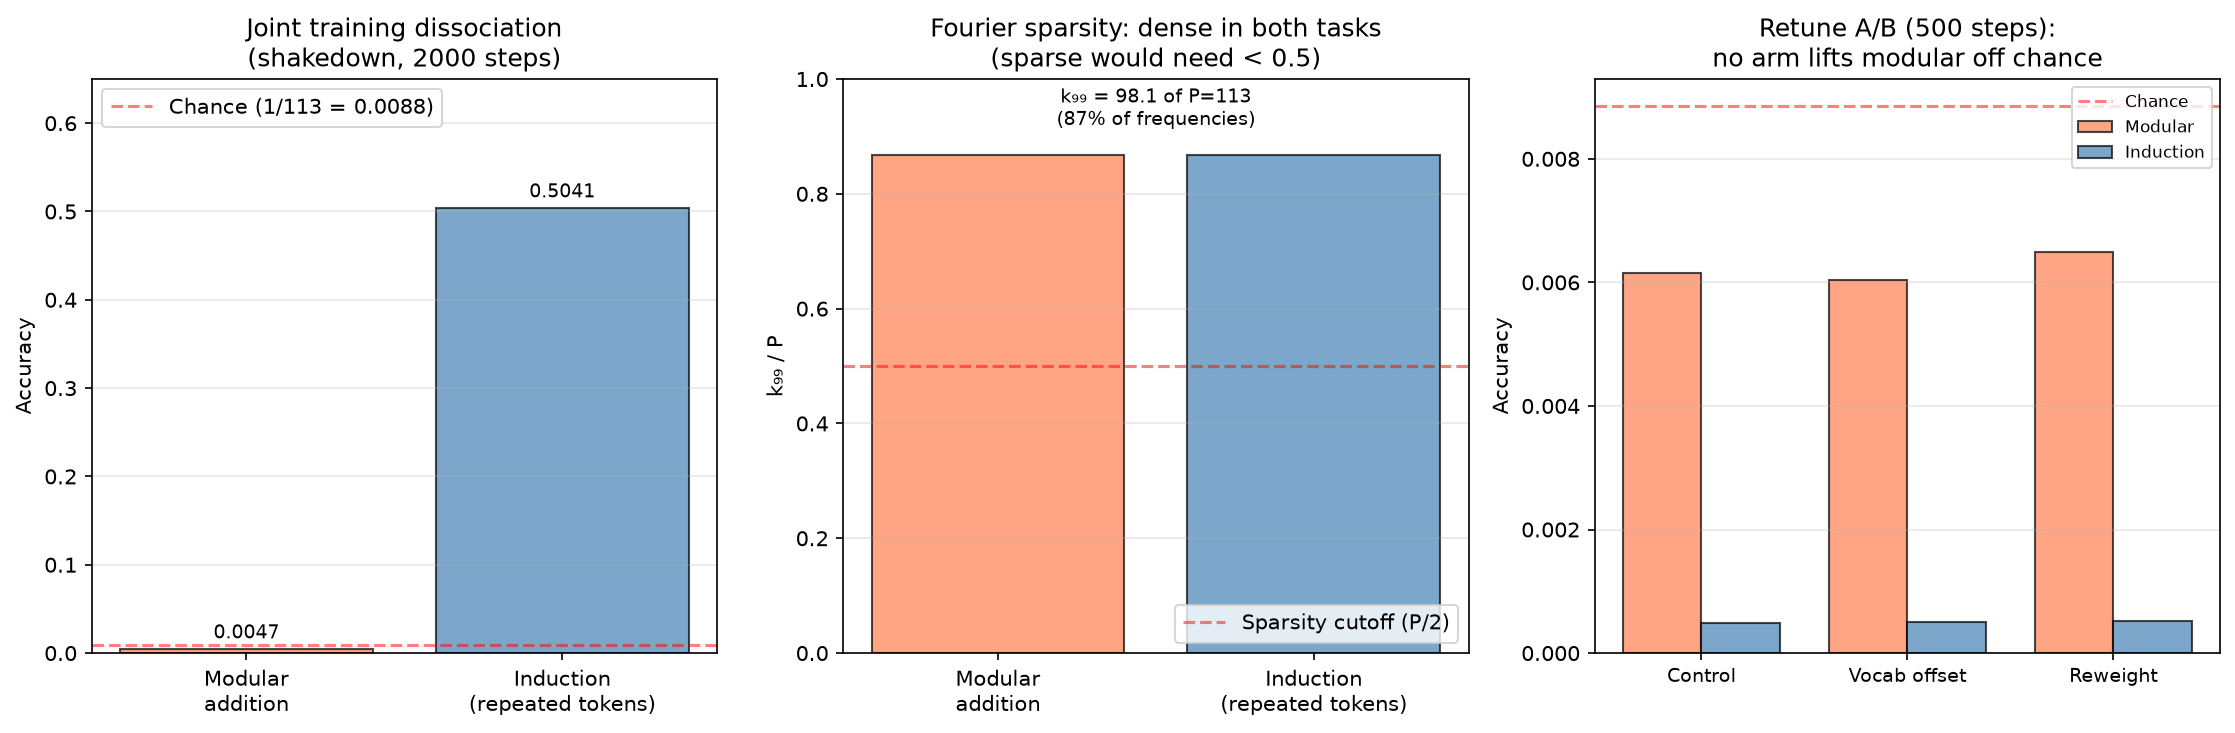
\includegraphics[width=0.95\textwidth]{../figures/joint_dissociation.png}
\caption{Joint dissociation (capstone shakedown). Modular stays at chance;
induction learns. Both Fourier dense under the energy criterion:
$k_{\mathrm{energy},90}=49/56$, sparse on 0/3 seeds.}
\label{fig:joint-dissociation}
% manifest: results/probe_capstone_shakedown.json
% manifest: results/capstone_20k_energy.json
\end{figure}

\subsection{Capstone 3$\times$20k run}
\label{sec:capstone-20k}
% manifest: results/capstone_20k.json

The capstone joint-training model (d\_model=256, 4 layers, 8 heads,
GPU, 3 seeds $\times$ 20,000 steps, configs/capstone.yaml) shows the
dissociation persists at full budget: induction accuracy
0.5034 $\pm$ 0.0002 --- the same plateau as the 2k-step shakedown
(0.5041), so structural, not a budget artifact --- and modular accuracy
0.1699 $\pm$ 0.0286, above chance (1/113 $\approx$ 0.0088) but far from
the solo-run 1.0. Its Fourier density is measured with the post-audit energy
criterion: $k_{\mathrm{energy},90}=49/56$ (of 56), energy\_sparse on 0/3
seeds -- the joint solution is \textbf{dense}, not a sparse Fourier circuit.
% manifest: results/capstone_20k_energy.json

\section{Limitations}
\label{sec:limitations}

\begin{itemize}
  \item \textbf{Micro-scale models:} findings may not transfer to larger
    (7B+) models. The capstone model is 4.3M parameters.
  \item \textbf{Algorithmic tasks:} modular addition and repeated tokens
    are cleaner than natural language; circuits found here may not be
    representative of circuits in language models.
  \item \textbf{No induction heads at standard scale:} the fixed-vs-fresh
    comparison (53.5\% val acc, 800 epochs) is the trustworthy scale for
    this paper; the standard-scale run with the corrected detector
    ($d_\text{model}=64$, 3000 epochs, three seeds) is the outstanding
    measurement, not a claim.
  \item \textbf{The head counts in this paper were retracted}
    (2026-10-19): the detectors measured the previous-token offset, so
    every ``$0 / N$'' figure was a statement about the detector. Even with
    the corrected detector, a perfectly periodic task cannot separate
    copying by content from copying by a fixed offset; only the
    dissociation probe can, and until it runs the wording is
    \emph{prefix-copying head}, not \emph{induction head}.
  \item \textbf{Grokking sparse circuit reproduced:} Rung 2 reached val
    accuracy 0.9999 $\pm$ 0.0002 with $k_{\mathrm{energy},90}$ = 5.7 $\pm$
    1.2 of 56 frequencies (sparse, 3/3 seeds) on both the Nanda-faithful and
    the historical protocol (GPU, 2026-10-14). The earlier NO-GROK label was
    an L1-mass metric artifact, retracted after the 2026-10-08 audit.
  \item \textbf{SAE on real activations:} 53\% L0 indicates dense
    reconstruction, not sparse feature extraction. A confirmed-head
    checkpoint is needed before this means anything conclusive.
  \item \textbf{Path patching unvalidated against a real head:}
    implementation is unit-tested only; end-to-end validation requires
    Rung 1's standard-scale work.
  \item \textbf{Single architecture family, limited seeds:} multi-seed
    harness covers Rungs 1--4; Rung 5 synthetic is single-seed; capstone
    shakedown is single-seed (3 seeds planned, 1 completed).
  \item \textbf{Attribution patching not implemented:} linear
    approximation with known failure modes on large activations
    (\citep{makelov2023subspace}).
  \item \textbf{Activation patching caveats:} layernorm denominator
    effects and subspace-projection illusions can mislead
    (\citep{makelov2023subspace}).
  \item \textbf{SAE interpretability is human-judged:} features can be
    illusory (\citep{makelov2023subspace}).
\end{itemize}

\section{Conclusion}
\label{sec:conclusion}

This work demonstrates a complete micro-scale MI pipeline: from-scratch
training, full instrumentation, causal circuit verification, and honest
negative reporting. The primary flagship, Rung 2 grokking modular addition,
is \textbf{reproduced} (val accuracy 0.9999 $\pm$ 0.0002, sparse Fourier
circuit with $k_{\mathrm{energy},90}$ = 5.7 $\pm$ 1.2 of 56, GPU, 3 seeds,
both protocols, 2026-10-14). The strongest verified result remains Rung 3's
superposition phase transition (root-caused, reproduced, multi-seed
manifest). The 2026-08-11 NO-GROK label was an L1-mass metric artifact,
retracted after the 2026-10-08 audit.

The capstone 3$\times$20k run reveals a dissociation under joint training
that persists at full budget: induction accuracy 0.5034 $\pm$ 0.0002,
modular accuracy 0.1699 $\pm$ 0.0286 (above chance, far from the solo-run
1.0). The honest negatives are contributions: NO-MOVE falsifies two
explanations of the joint-training dissociation at this scale; the P=59
positive control carries the same L1 metric defect and is marked
metric-suspect.

\bibliographystyle{plainnat}
\bibliography{references}

\end{document}